\documentclass{standalone}
\usepackage{tikz}
\usepackage{ctex,siunitx,ninecolors}
\usepackage{tkz-euclide}
\usepackage{amsmath}
\usetikzlibrary{patterns, calc}
\usetikzlibrary {decorations.pathmorphing, decorations.pathreplacing, decorations.shapes,}
\begin{document}
\small
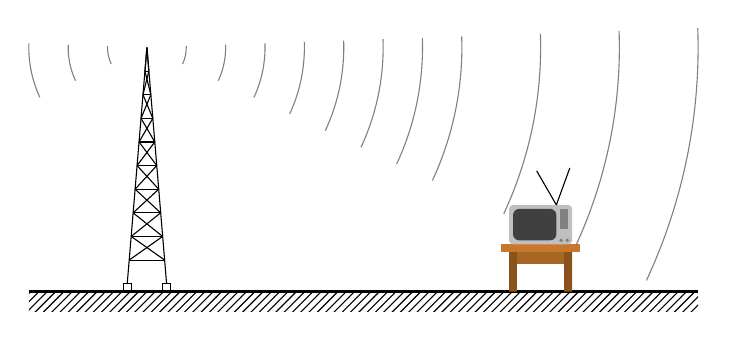
\begin{tikzpicture}[>=stealth]
  \foreach \x in {0.5,1,...,4,5,6,7} { \draw[gray] (2:\x)arc(2:-25:\x); }
  \foreach \x in {0.5,1,1.5} { \draw[gray](178:\x)arc(178:205:\x); }
  \draw(-0.25,-3)--(0,0)--(0.25,-3);
  \foreach \x in {-2.7,-2.4,...,-0.2}
  {
    \draw(-\x/3*0.25,\x)--(\x/3*0.25,\x);
    \draw(-\x/3*0.25,\x)--(\x/3*0.25+0.025,\x+0.3);
    \draw(-\x/3*0.25-0.025,\x+0.3)--(\x/3*0.25,\x);
  }
  \draw(-0.3,-3)rectangle(-0.2,-3.1)(0.3,-3)rectangle(0.2,-3.1);
  \fill[pattern= north east lines](-1.5,-3.1)rectangle(7,-3.35);
  \draw[thick](-1.5,-3.1)--(7,-3.1);
  \fill[brown6](4.5,-2.6)rectangle(5.5,-2.5);
  \fill[brown4](4.7,-2.6)rectangle(4.6,-3.1)(5.3,-2.6)rectangle(5.4,-3.1);
  \fill[brown5](4.7,-2.6)rectangle(5.3,-2.75);
  \fill[lightgray,rounded corners=0.5mm](4.6,-2.5)rectangle(5.4,-2.0);
  \fill[darkgray,rounded corners=0.8mm](4.65,-2.45)rectangle(5.2,-2.05);
  \fill[gray](5.25,-2.05)rectangle(5.35,-2.3);
  \fill[gray](5.26,-2.45)circle(0.7pt)(5.34,-2.45)circle(0.7pt);
  \draw(5.2,-2.0)--++(120:0.5)(5.2,-2.0)--++(70:0.5);
\end{tikzpicture}
\end{document}